\PassOptionsToPackage{unicode}{hyperref}
\documentclass[aspectratio=1610, professionalfonts, 9pt]{beamer}

\usefonttheme[onlymath]{serif}
\usetheme[showtotalframes]{tudo}


\usepackage{polyglossia}
\setmainlanguage{english}

% Mathematik
\usepackage{mathtools}

% Enable Unicode-Math and follow the ISO-Standards for typesetting math
\usepackage[
  math-style=ISO,
  bold-style=ISO,
  sans-style=italic,
  nabla=upright,
  partial=upright,
]{unicode-math}
\setmathfont{Latin Modern Math}

% nice, small fracs for the text with \sfrac{}{}
\usepackage{xfrac}

\usepackage{multicol}
\usepackage{graphicx}
\usepackage{amssymb}
\usepackage{amsmath}
\usepackage{xparse}
\usepackage{braket}
\usepackage{units}
\usepackage[locale=DE,separate-uncertainty=true,per-mode=reciprocal,output-decimal-marker={,},]{siunitx}
\sisetup{
  round-mode          = places, % Rounds numbers
  round-precision     = 2, % to 2 places
}
\usepackage[section]{placeins}
\usepackage{pdflscape}
\usepackage{expl3}
\usepackage{bookmark}
\usepackage{booktabs}
%Komma als Dezimaltrenner in der mathe Umgebung, um in Umgebungen wie [0, 2] ein Leerzeichen nach dem Komma zu erhalten einfach eins setzen
\usepackage{icomma}
\usepackage{cancel}

\usepackage[
  backend=biber,   % use modern biber backend
  autolang=hyphen, % load hyphenation rules for if language of bibentry is not
                   % german, has to be loaded with \setotherlanguages
                   % in the references.bib use langid={en} for english sources
]{biblatex}
\addbibresource{references.bib}  % die Bibliographie einbinden
\DefineBibliographyStrings{german}{andothers = {{et\,al\adddot}}}



\usepackage{hyperref}
\usepackage{subfigure}
\usepackage[labelformat=empty]{caption}





%%%%%%%%%%%%%%%%%%%%%%%%%%%%%%%%%%%%%%%%%%%%%%%%%%%%%%%%%%%%%%%%%%%%%%%%%%%%%%%%
%%%%%-------------Hier Titel/Autor/Grafik/Lehrstuhl eintragen--------------%%%%%
%%%%%%%%%%%%%%%%%%%%%%%%%%%%%%%%%%%%%%%%%%%%%%%%%%%%%%%%%%%%%%%%%%%%%%%%%%%%%%%%

%Titel:
\title{Detektion von Fake News}
%Title graphic:
\titlegraphic{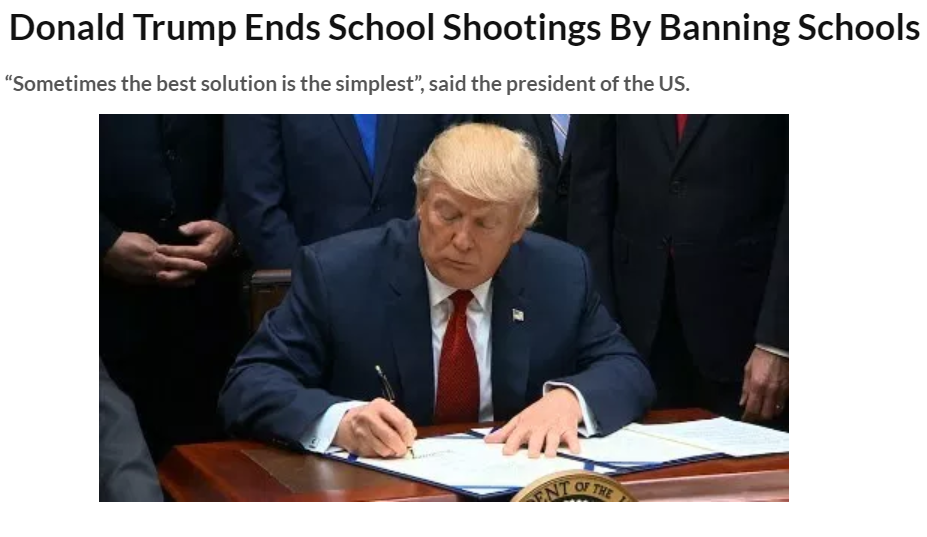
\includegraphics[height=.5\textheight]{pictures/title_fake_news.PNG}}
%Autor
\author{%
  Clemens Vorsmann \& \\ 
  %\texorpdfstring{\and}{, }%
  Lars Möllerherm
  %
}
%Lehrstuhl/Fakultät
\institute{Fakultät Physik}

\AtBeginSection[]{
    \begin{frame}
      \vfill
      \centering
      \usebeamerfont{title}\insertsectionhead\par%
      \vfill
    \end{frame}
}

\begin{document}

  \begin{frame}
    \titlepage
  \end{frame}

  \begin{frame}
    \frametitle{Methode und Modell}
    \begin{columns}
      \column{0.3\textwidth}
      \begin{figure}
        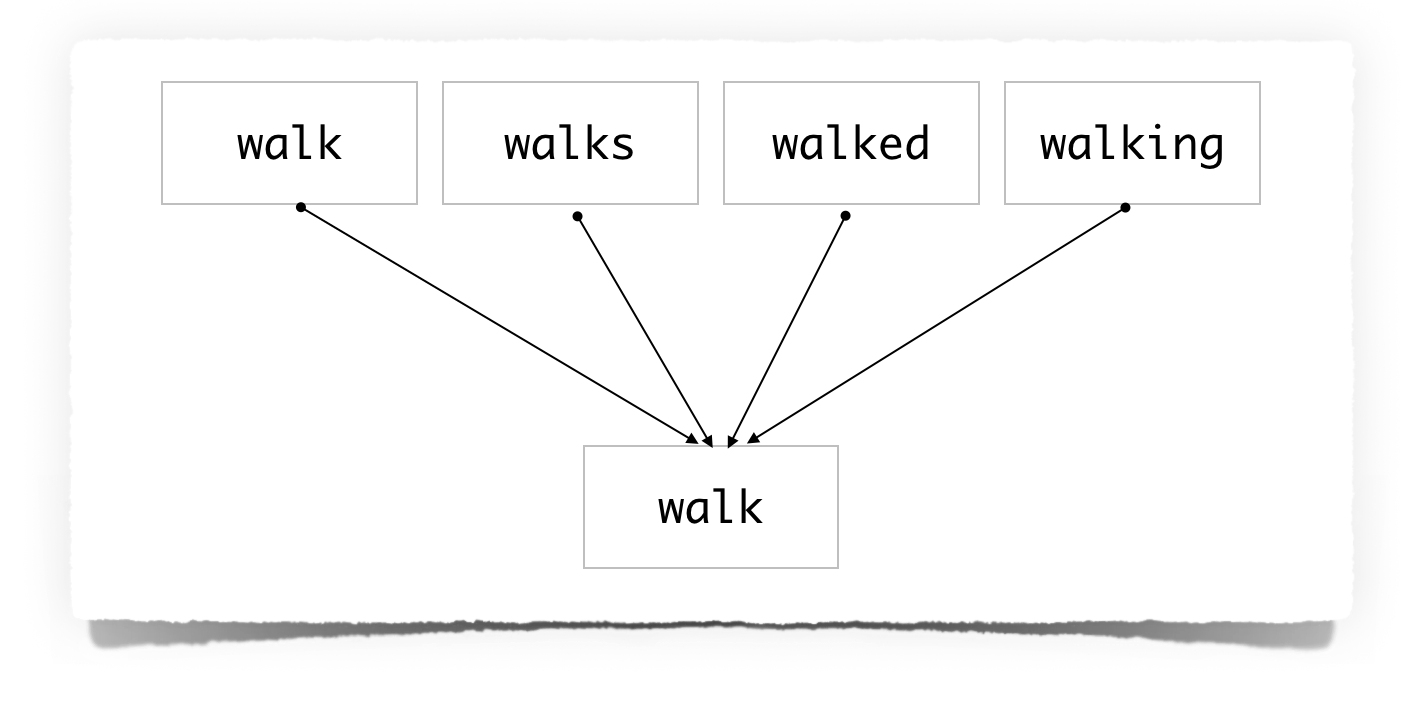
\includegraphics[width=\textwidth]{pictures/lemma.png}
        \caption{Lemmatisierung \cite{lemma}}
      \end{figure}  
      \begin{figure}
          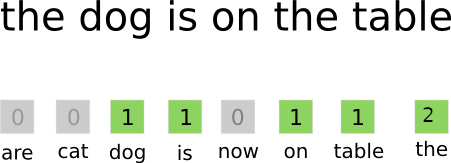
\includegraphics[width=\textwidth]{pictures/bow_schematisch.png}
          \caption{Bag of Words Modell \cite{bow_pic}}
          \label{}
      \end{figure}
      \column{0.25\textwidth}
      \begin{figure}
          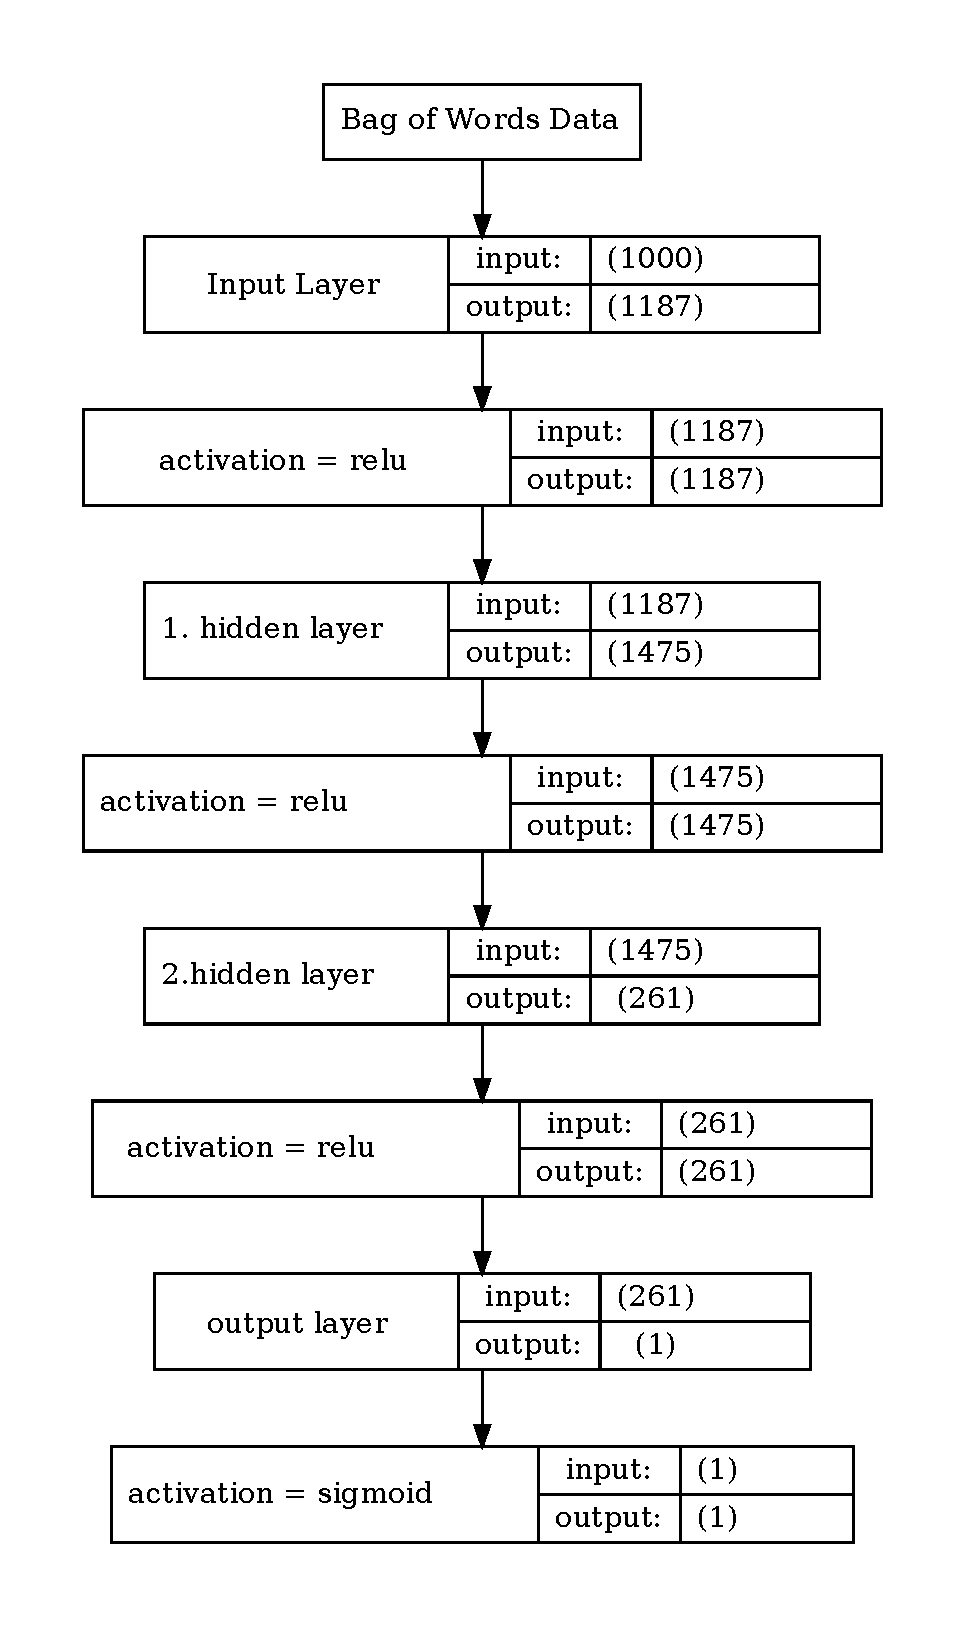
\includegraphics[width=\textwidth]{pictures/bow/opt_model_bow2.pdf}
          \caption{}
          \label{}
      \end{figure}
      
    \end{columns}
  \end{frame}

  \begin{frame}
    \frametitle{Training}
    \begin{columns}
      \column{0.5\textwidth}
      \begin{figure}
          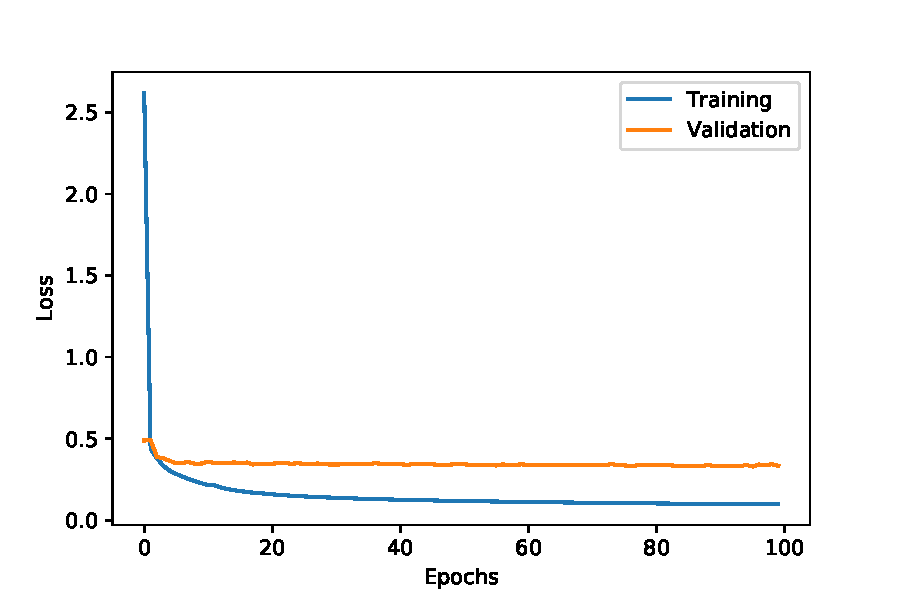
\includegraphics[width=\textwidth]{pictures/bow/history_bow_best.pdf}
          \caption{}
          \label{}
      \end{figure}
      
      \column{0.5\textwidth}
      \begin{figure}
          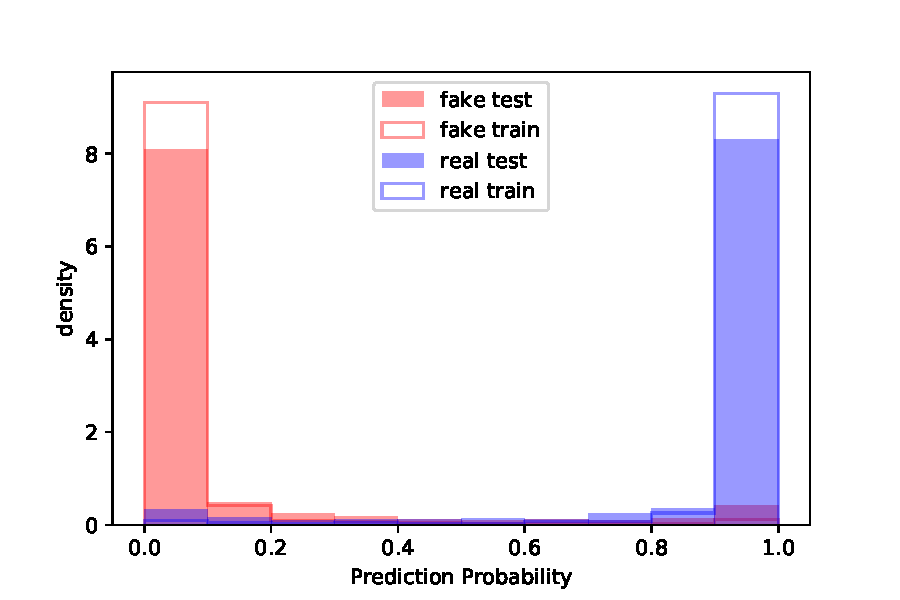
\includegraphics[width=\textwidth]{pictures/bow/prob_bow_best_nn.pdf}
          \caption{}
          \label{}
      \end{figure}
      
    \end{columns}
  \end{frame}

  \begin{frame}
    \frametitle{Performance}
    \begin{columns}
      \column{0.5\textwidth}
      \begin{figure}
          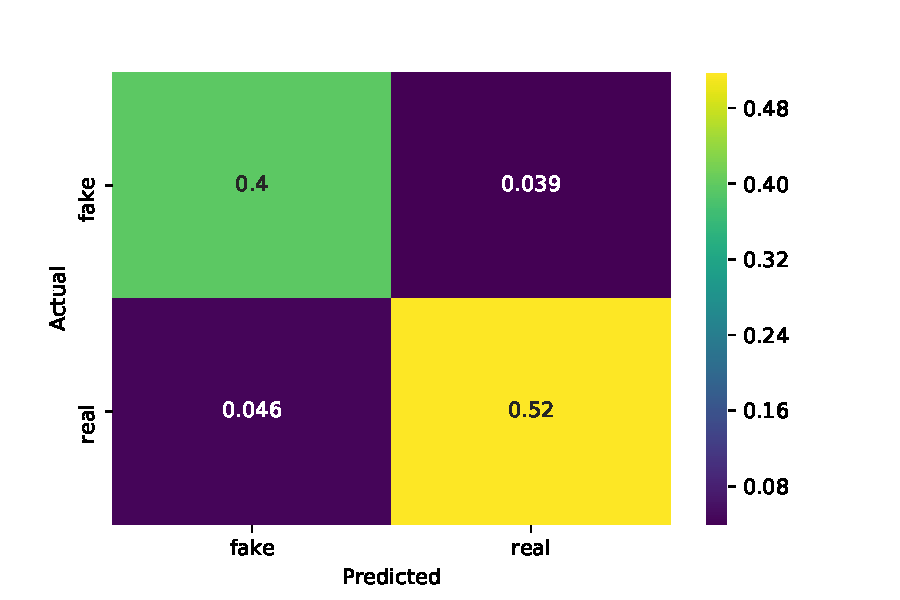
\includegraphics[width=\textwidth]{pictures/bow/cnfsn_mtx_bow_best_nn.pdf}
          \caption{}
          \label{}
      \end{figure}

      \column{0.5\textwidth}
      \begin{figure}
          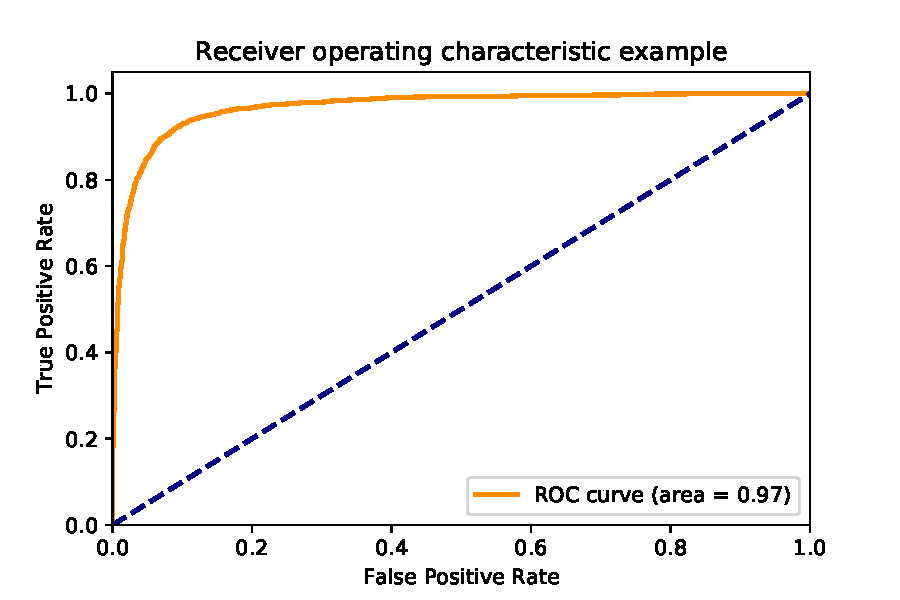
\includegraphics[width=\textwidth]{pictures/bow/roc_Hyperopt_bow_best_nn.pdf}
          \caption{}
          \label{}
      \end{figure}
    \end{columns}
  \end{frame}

  \begin{frame}
    \frametitle{Interpretation der Confusion Matrix}
    \begin{figure}
      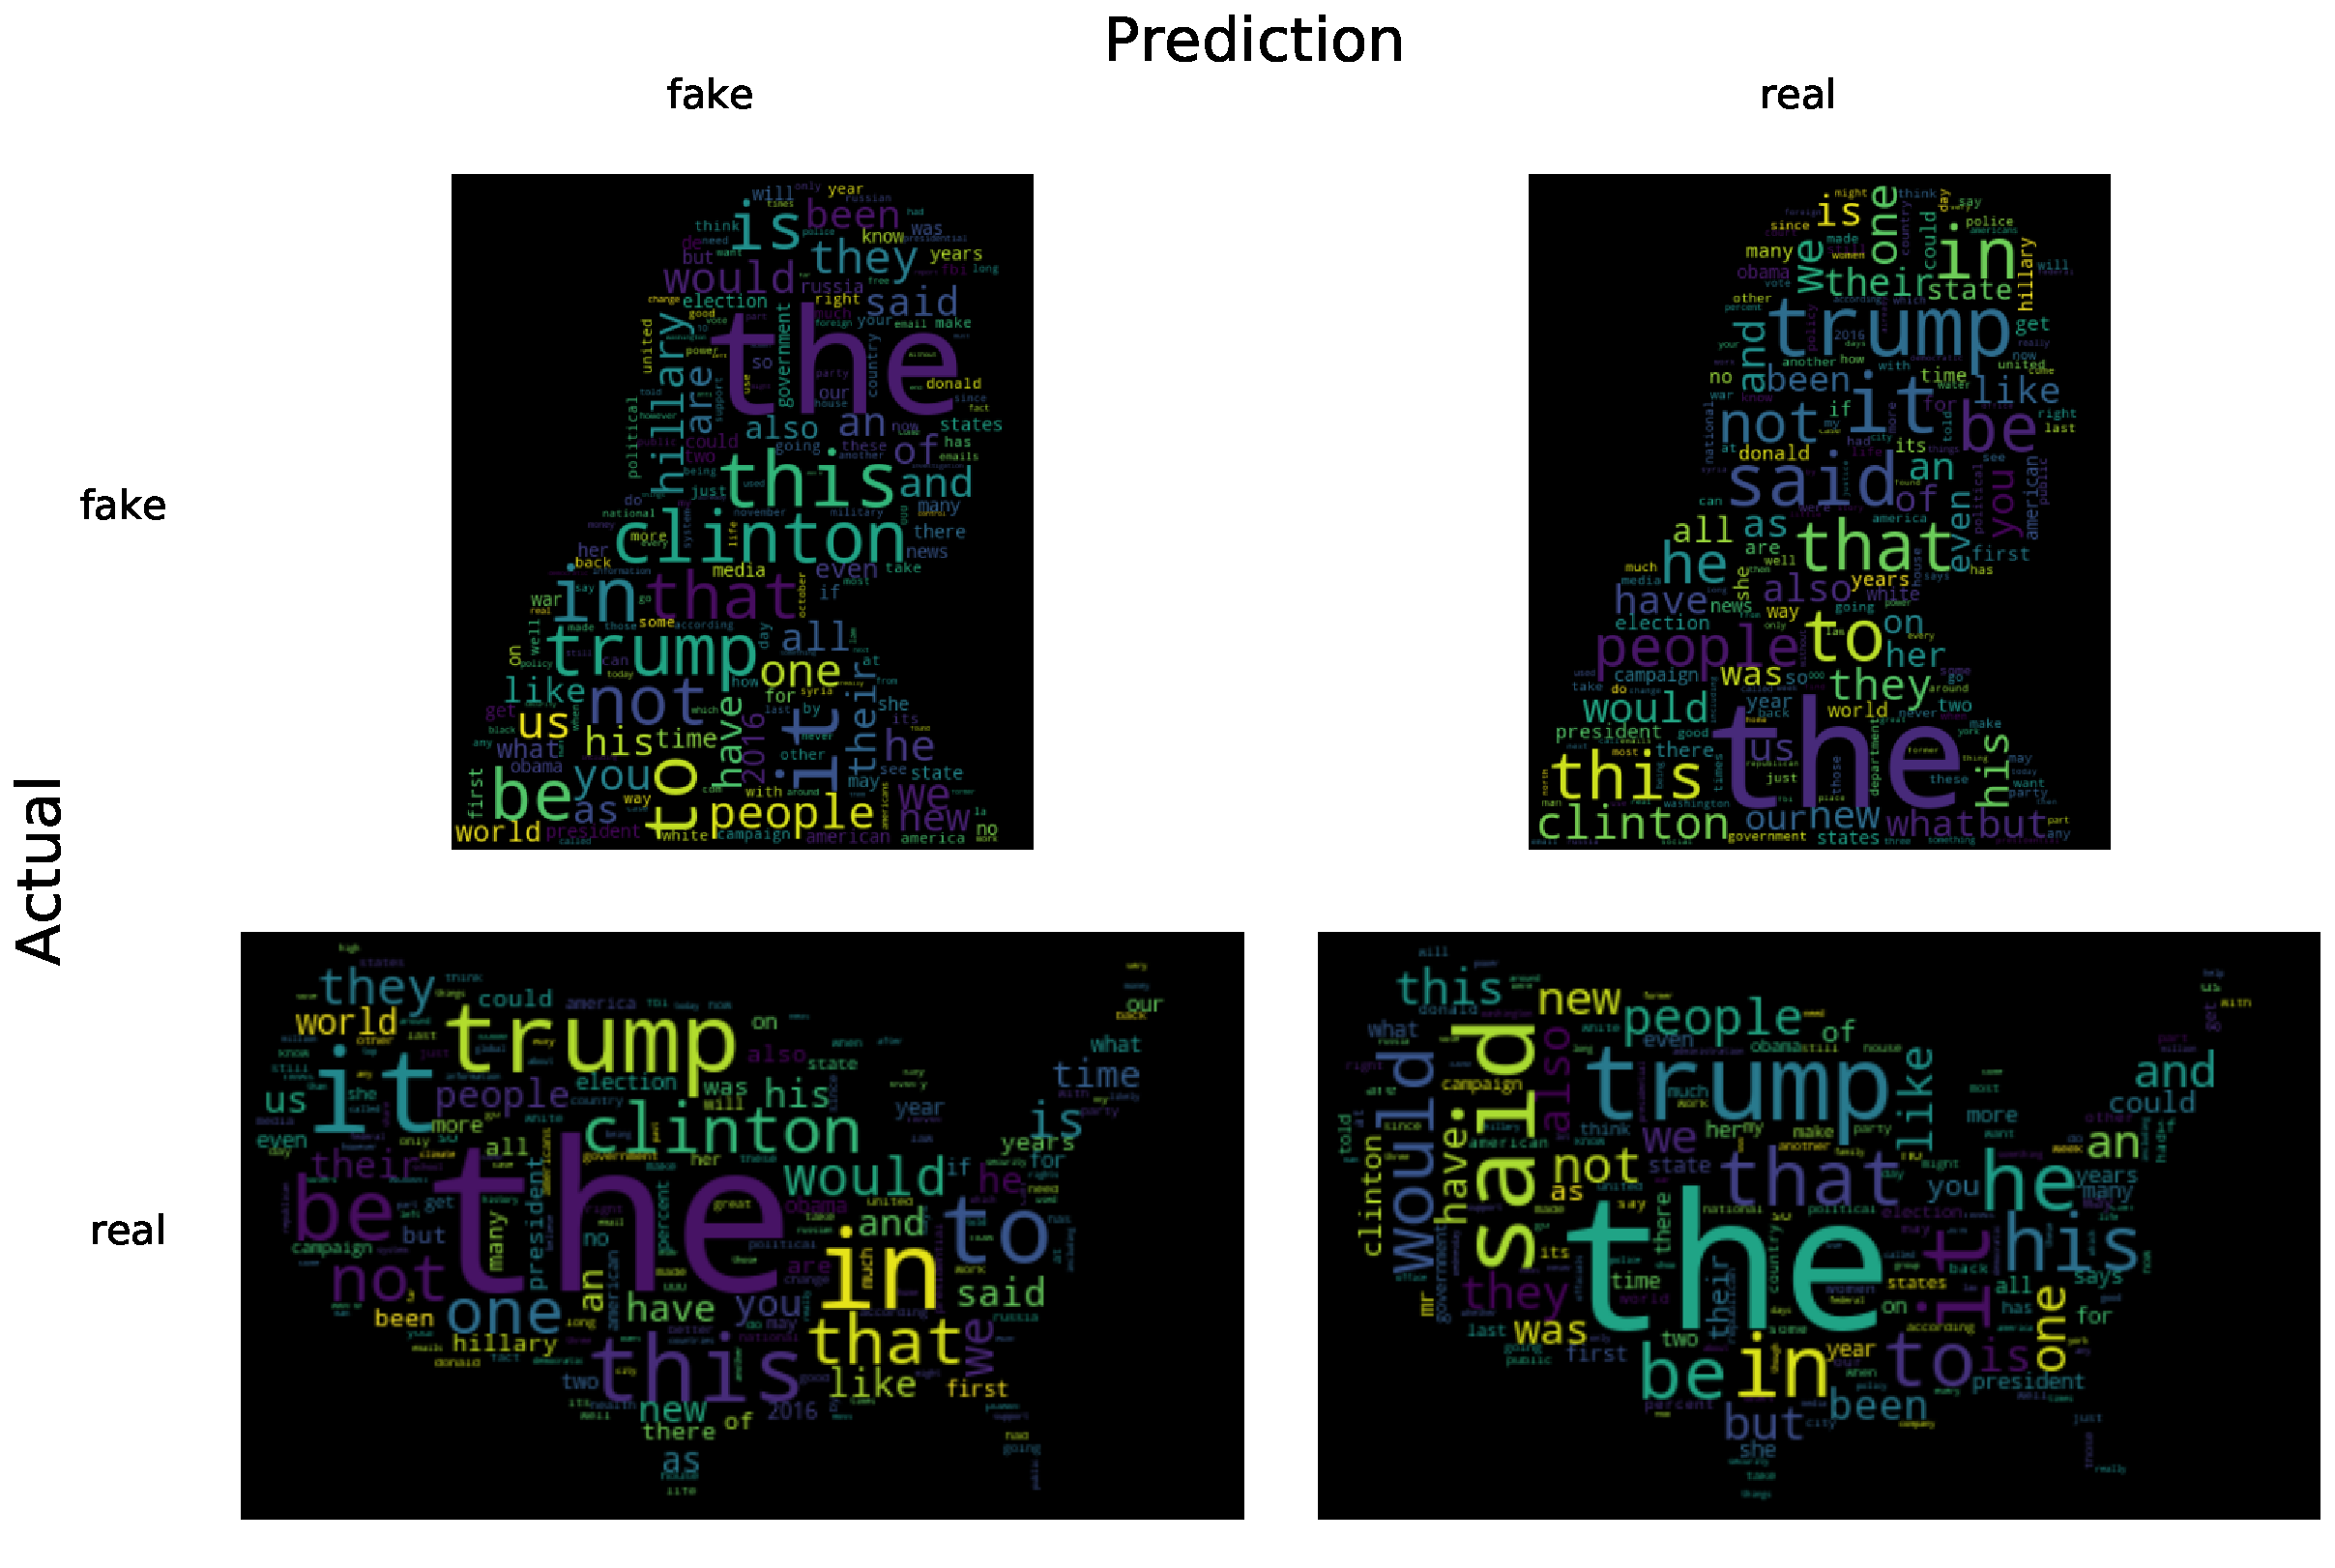
\includegraphics[width=0.7\textwidth]{pictures/bow/cnfn_wordcloud.pdf}
      \caption{}
      \label{}
    \end{figure}
  \end{frame}

  \begin{frame}
    \frametitle{Vergleichsmethode}
    \begin{figure}
      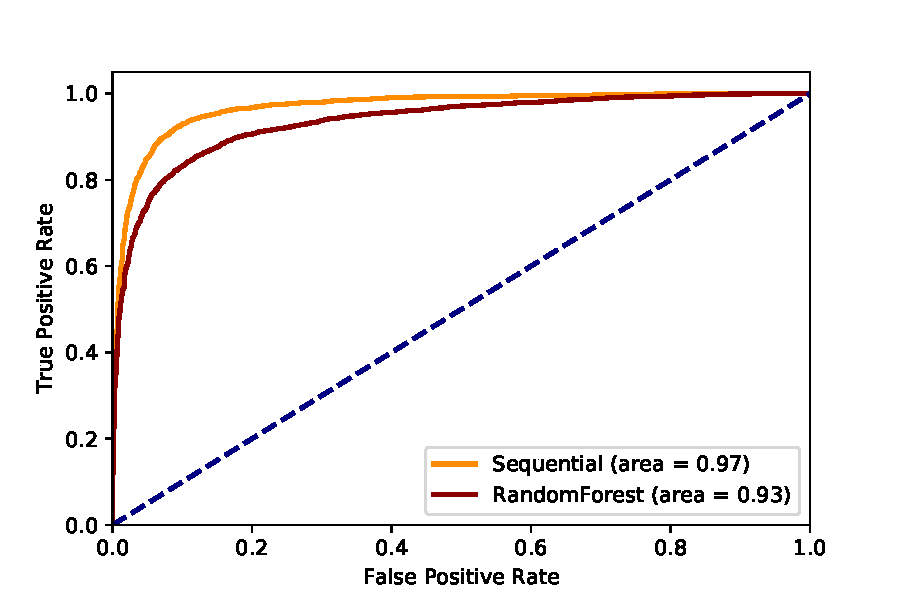
\includegraphics[width=0.7\textwidth]{pictures/bow/roc_comparison.pdf}
      \caption{}
      \label{}
    \end{figure}
  \end{frame}

  \begin{frame}
    \vfill
    \centering
    \begin{beamercolorbox}[sep=8pt,center,shadow=false,rounded=true]{title}
      \huge{\textbf{Vielen Dank für Ihre Aufmerksamkeit}}
    \end{beamercolorbox}
  \end{frame}

\section{Back Up Folien}

  \begin{frame}
    \frametitle{Wordclouds}
    \begin{columns}
      \column{0.5\textwidth}
      \begin{figure}
          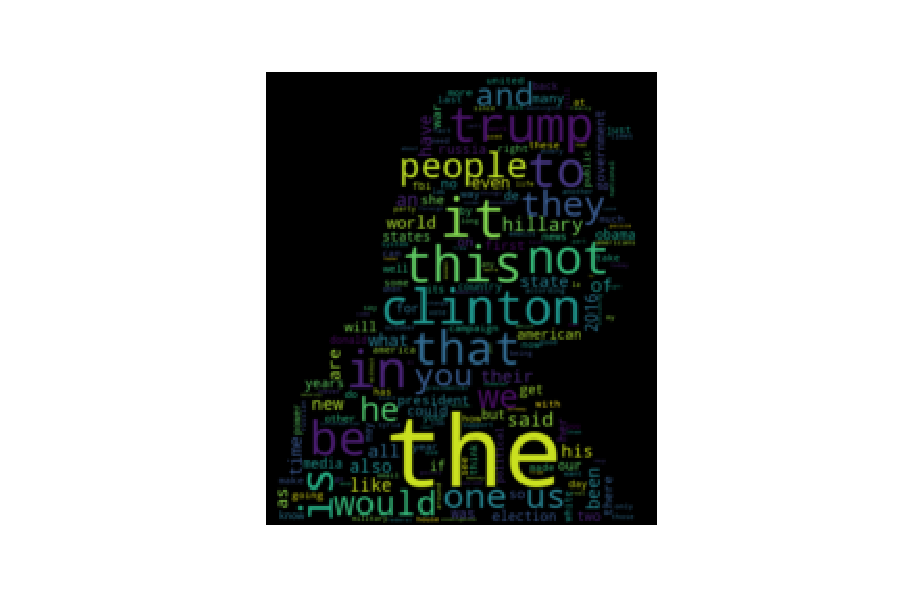
\includegraphics[width=\textwidth]{pictures/fake_wordcloud.pdf}
          \caption{Fake News}
          \label{}
      \end{figure}

      \column{0.5\textwidth}
      \begin{figure}
          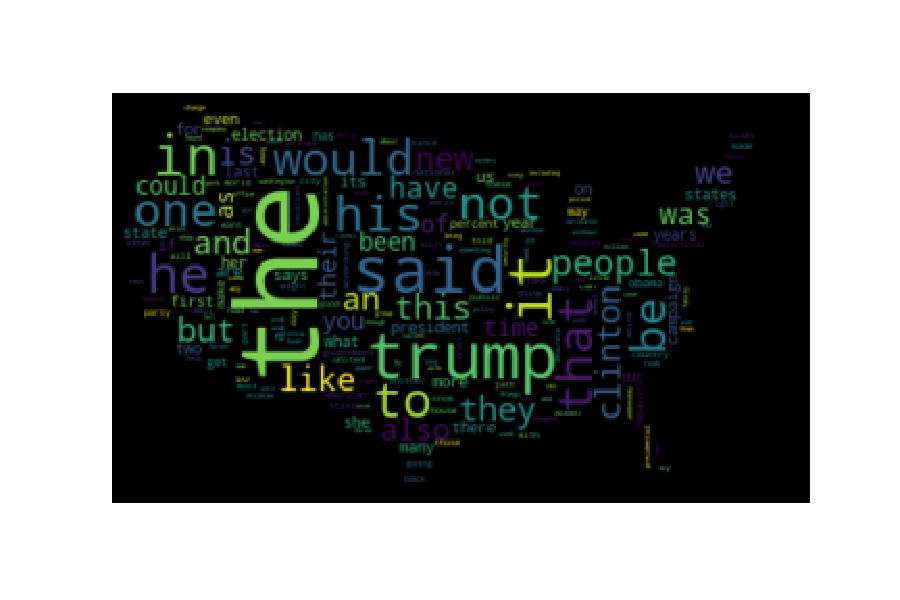
\includegraphics[width=\textwidth]{pictures/real_wordcloud.pdf}
          \caption{Real News}
          \label{}
      \end{figure}
    \end{columns}
  \end{frame}

  \begin{frame}
    \frametitle{Interpretation der Gewichte}
    \begin{figure}
          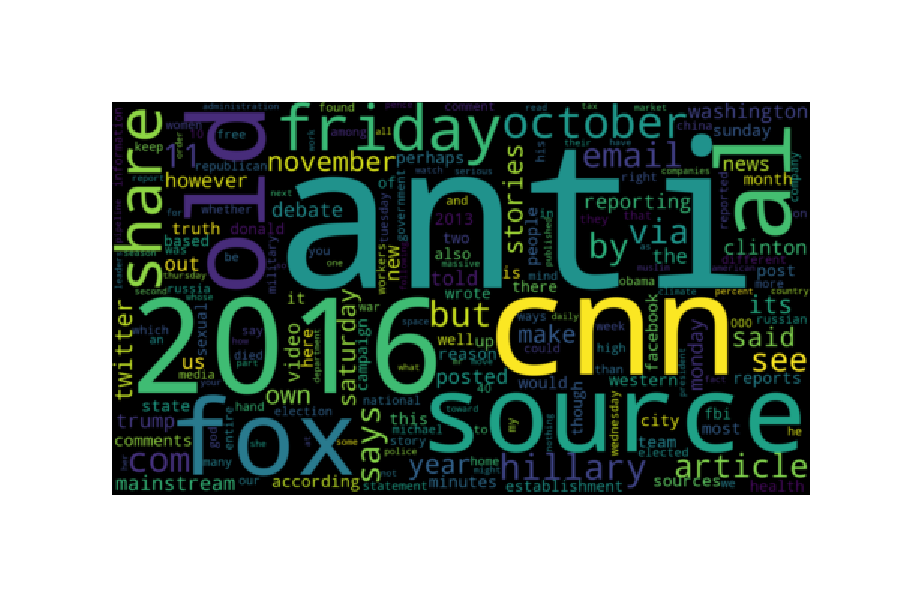
\includegraphics[width=0.8\textwidth]{pictures/bow/weights_wordcloud.pdf}
          \caption{}
          \label{}
      \end{figure}
  \end{frame}

  \begin{frame}
    \frametitle{Performance des Random Forests}
    \begin{columns}
      \column{0.5\textwidth}
      \begin{figure}
          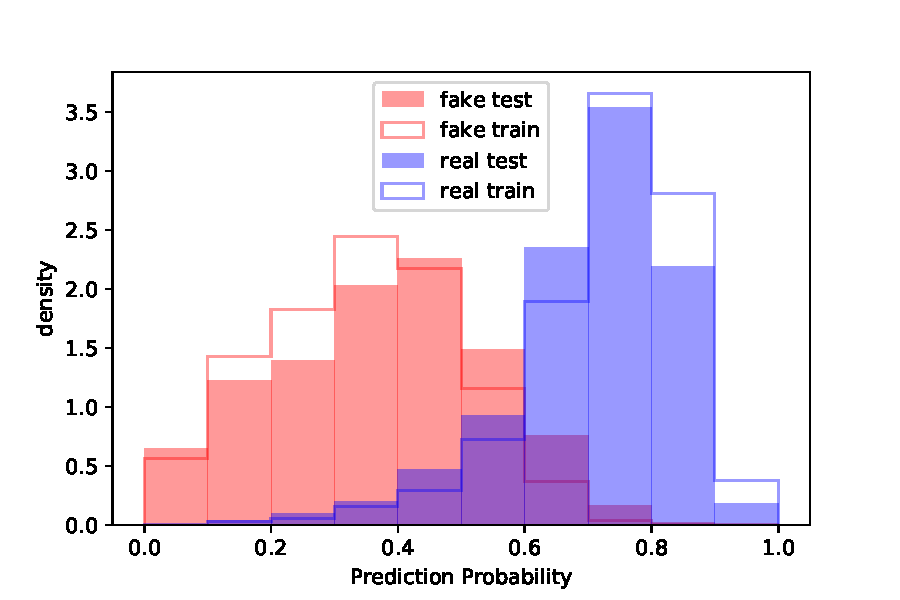
\includegraphics[width=\textwidth]{pictures/bow/RF/prob_bow_best_nn.pdf}
          \caption{}
          \label{}
      \end{figure}

      \column{0.5\textwidth}
      \begin{figure}
          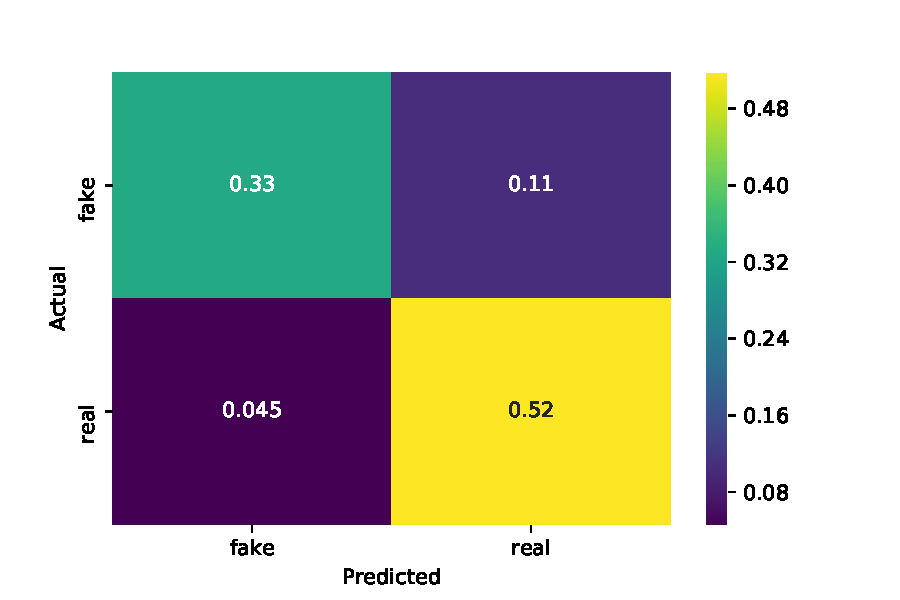
\includegraphics[width=\textwidth]{pictures/bow/RF/cnfsn_mtx_bow_best_nn.pdf}
          \caption{}
          \label{}
      \end{figure}
    \end{columns}
  \end{frame}

  \begin{frame}
    \begin{figure}
        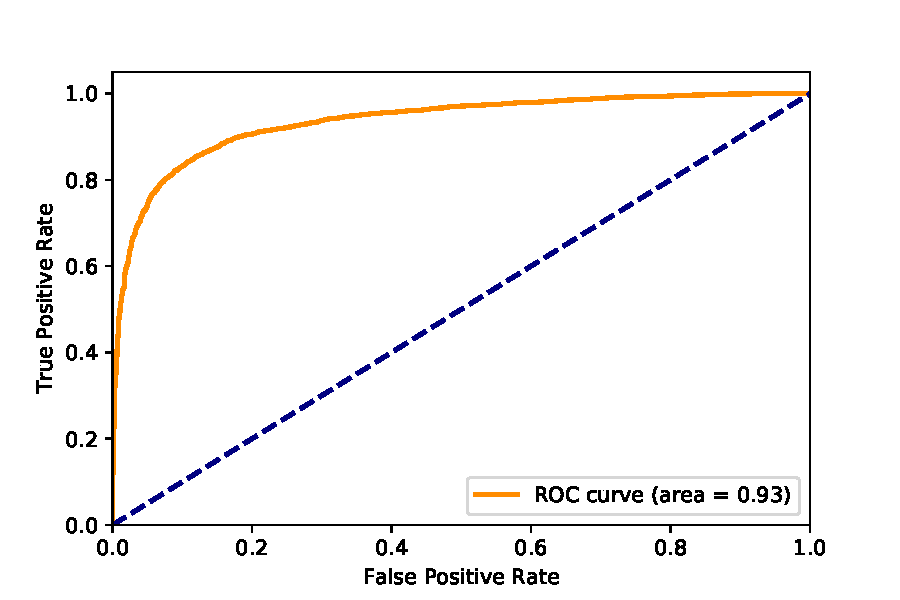
\includegraphics[width=0.7\textwidth]{pictures/bow/RF/roc_Hyperopt_bow_best_nn.pdf}
        \caption{}
        \label{}
    \end{figure}
  \end{frame}
  \begin{frame}
    \begin{figure}
        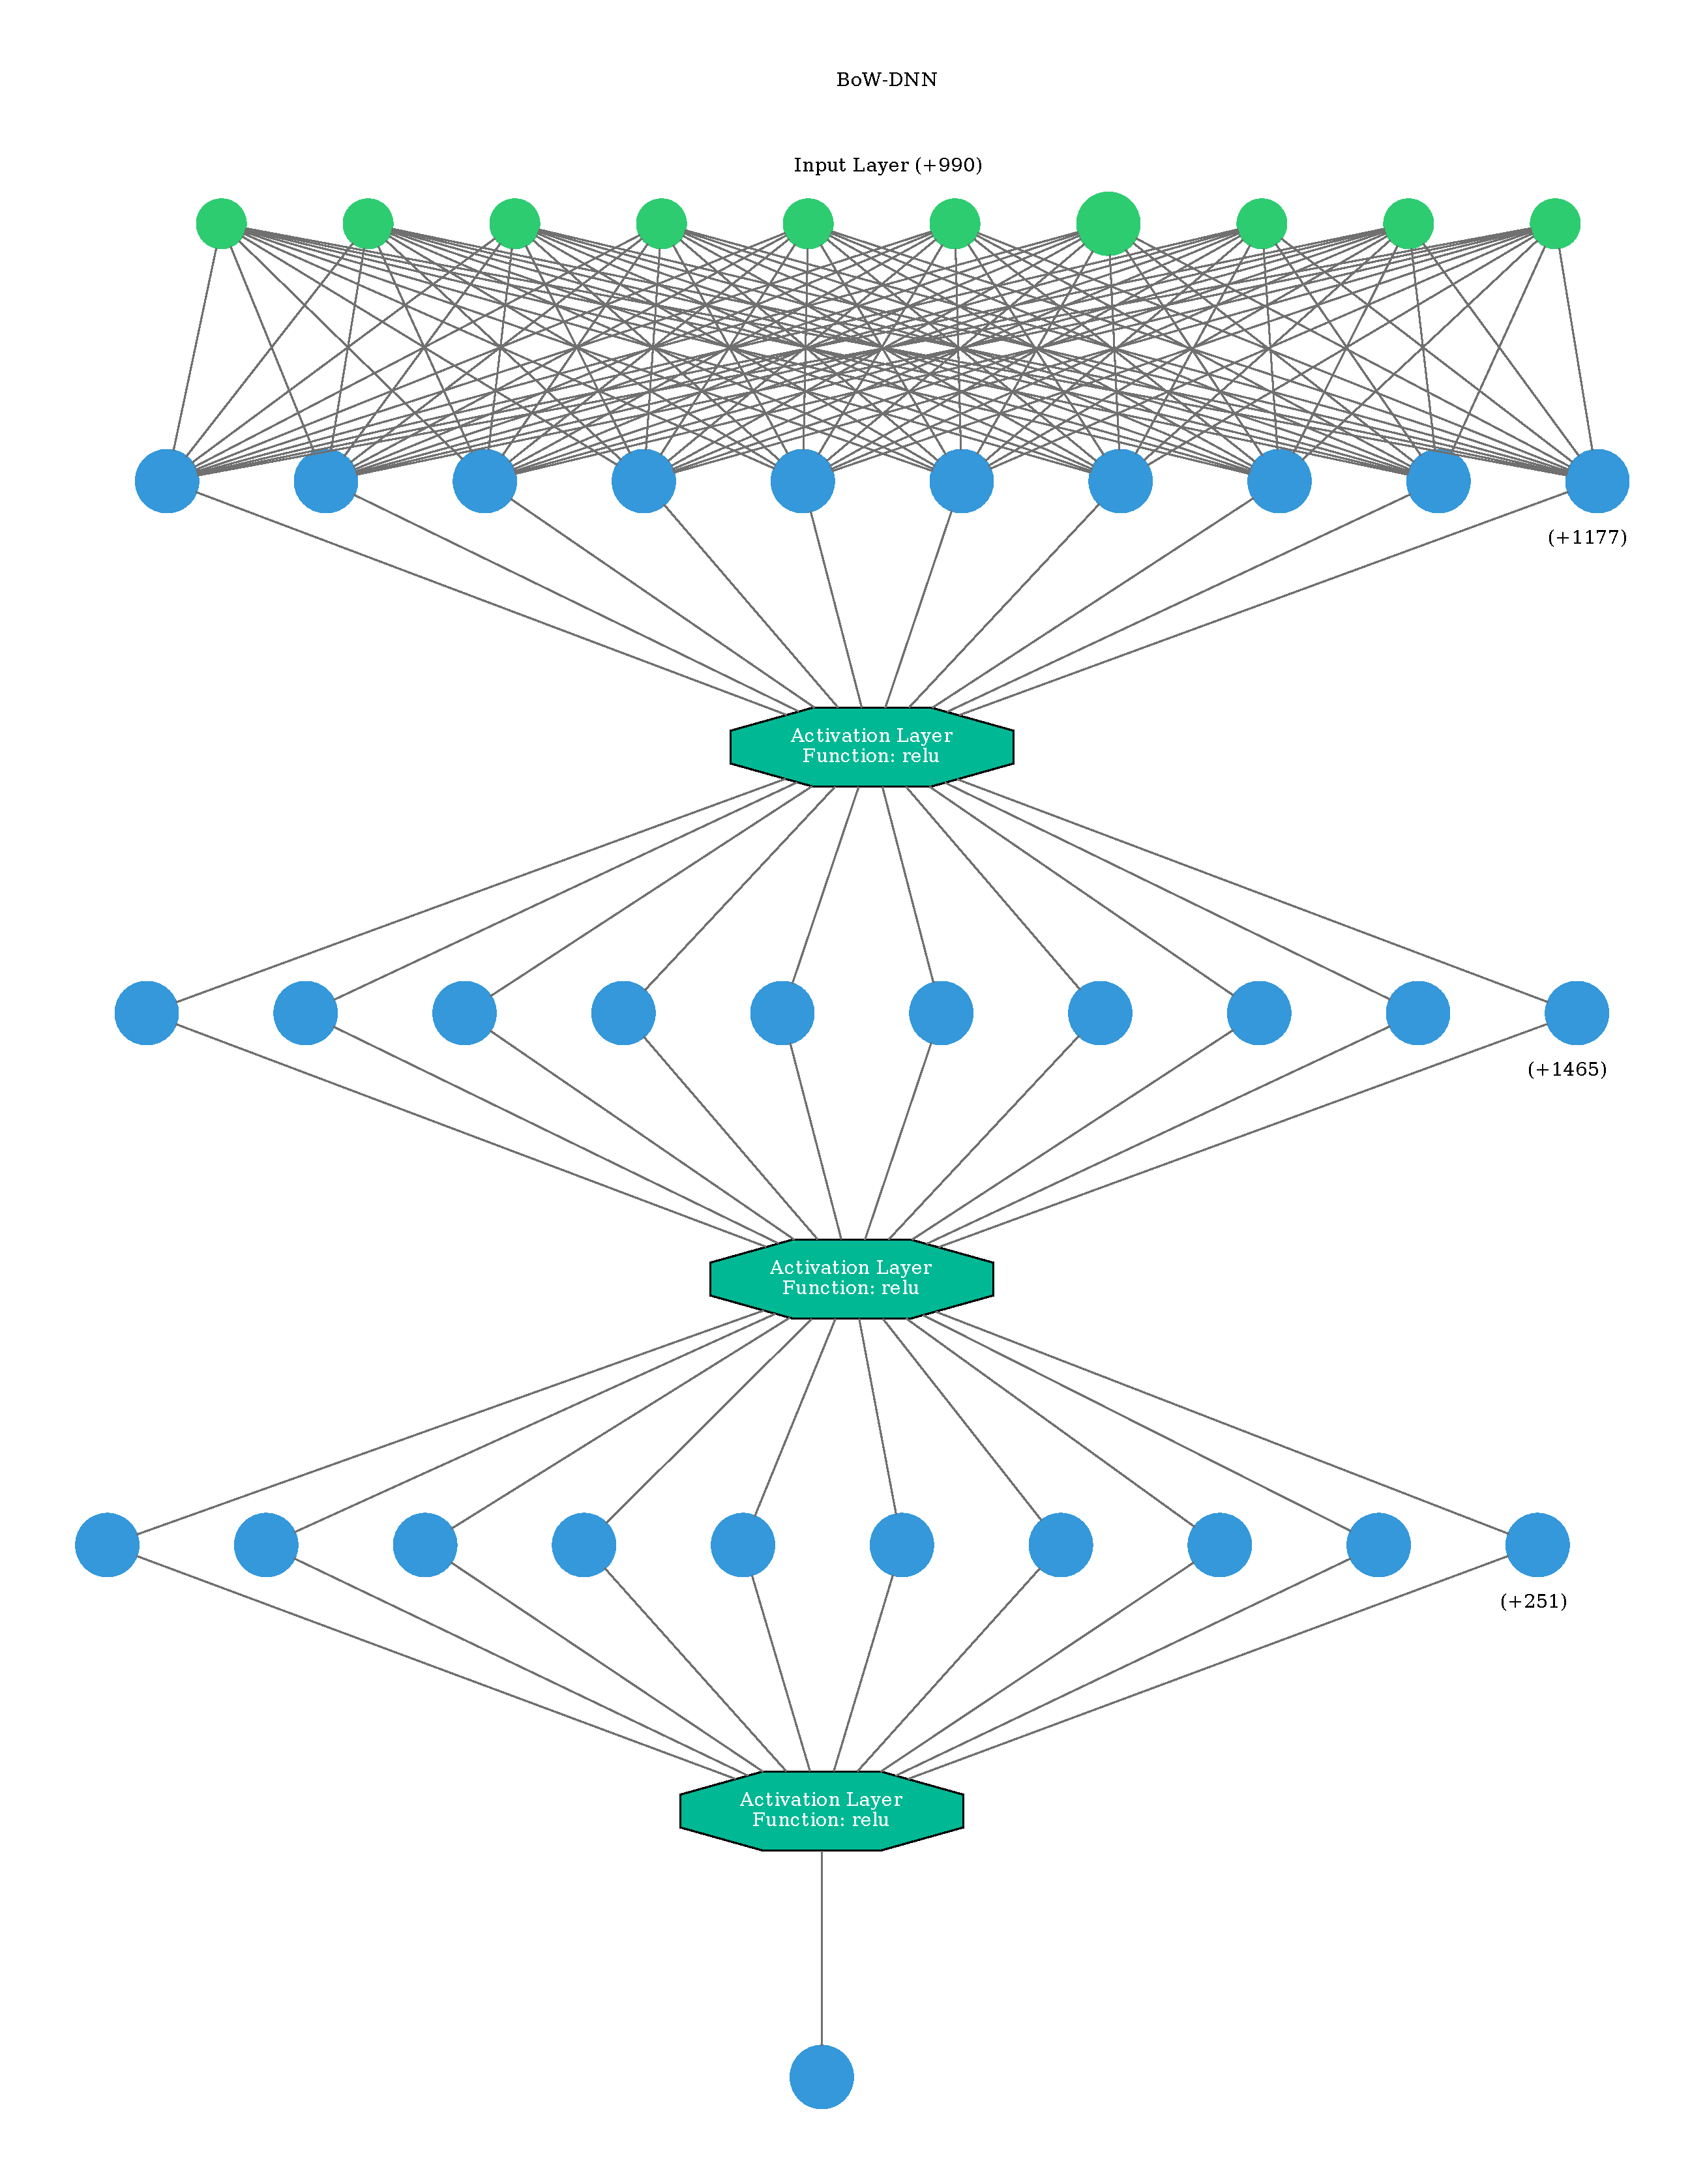
\includegraphics[angle=90,width=0.7\textwidth]{pictures/bow/bow_dnn_graph.pdf}
        \caption{}
        \label{}
    \end{figure}
  \end{frame}
  \begin{frame}
    \printbibliography
  \end{frame}
\end{document}